\newenvironment{Shaded}{}{}
\newcommand{\AlertTok}[1]{\textcolor[rgb]{1.00,0.00,0.00}{\textbf{#1}}}
\newcommand{\AnnotationTok}[1]{\textcolor[rgb]{0.38,0.63,0.69}{\textbf{\textit{#1}}}}
\newcommand{\AttributeTok}[1]{\textcolor[rgb]{0.49,0.56,0.16}{#1}}
\newcommand{\BaseNTok}[1]{\textcolor[rgb]{0.25,0.63,0.44}{#1}}
\newcommand{\BuiltInTok}[1]{#1}
\newcommand{\CharTok}[1]{\textcolor[rgb]{0.25,0.44,0.63}{#1}}
\newcommand{\CommentTok}[1]{\textcolor[rgb]{0.38,0.63,0.69}{\textit{#1}}}
\newcommand{\CommentVarTok}[1]{\textcolor[rgb]{0.38,0.63,0.69}{\textbf{\textit{#1}}}}
\newcommand{\ConstantTok}[1]{\textcolor[rgb]{0.53,0.00,0.00}{#1}}
\newcommand{\ControlFlowTok}[1]{\textcolor[rgb]{0.00,0.44,0.13}{\textbf{#1}}}
\newcommand{\DataTypeTok}[1]{\textcolor[rgb]{0.56,0.13,0.00}{#1}}
\newcommand{\DecValTok}[1]{\textcolor[rgb]{0.25,0.63,0.44}{#1}}
\newcommand{\DocumentationTok}[1]{\textcolor[rgb]{0.73,0.13,0.13}{\textit{#1}}}
\newcommand{\ErrorTok}[1]{\textcolor[rgb]{1.00,0.00,0.00}{\textbf{#1}}}
\newcommand{\ExtensionTok}[1]{#1}
\newcommand{\FloatTok}[1]{\textcolor[rgb]{0.25,0.63,0.44}{#1}}
\newcommand{\FunctionTok}[1]{\textcolor[rgb]{0.02,0.16,0.49}{#1}}
\newcommand{\ImportTok}[1]{#1}
\newcommand{\InformationTok}[1]{\textcolor[rgb]{0.38,0.63,0.69}{\textbf{\textit{#1}}}}
\newcommand{\KeywordTok}[1]{\textcolor[rgb]{0.00,0.44,0.13}{\textbf{#1}}}
\newcommand{\NormalTok}[1]{#1}
\newcommand{\OperatorTok}[1]{\textcolor[rgb]{0.40,0.40,0.40}{#1}}
\newcommand{\OtherTok}[1]{\textcolor[rgb]{0.00,0.44,0.13}{#1}}
\newcommand{\PreprocessorTok}[1]{\textcolor[rgb]{0.74,0.48,0.00}{#1}}
\newcommand{\RegionMarkerTok}[1]{#1}
\newcommand{\SpecialCharTok}[1]{\textcolor[rgb]{0.25,0.44,0.63}{#1}}
\newcommand{\SpecialStringTok}[1]{\textcolor[rgb]{0.73,0.40,0.53}{#1}}
\newcommand{\StringTok}[1]{\textcolor[rgb]{0.25,0.44,0.63}{#1}}
\newcommand{\VariableTok}[1]{\textcolor[rgb]{0.10,0.09,0.49}{#1}}
\newcommand{\VerbatimStringTok}[1]{\textcolor[rgb]{0.25,0.44,0.63}{#1}}
\newcommand{\WarningTok}[1]{\textcolor[rgb]{0.38,0.63,0.69}{\textbf{\textit{#1}}}}

\chapter{Desarrollo del Proyecto}
% [Este capítulo se considera el más importante al elaborar el proyecto de titulación. Se describe el procedimiento seguido para lograr el objetivo planteado. Se explica qué y cómo se hizo, además se debe de convencer de que los métodos o procedimientos usados fueron los más adecuados.

% Deben detallarse los procedimientos, técnicas, métodos, metodologías y demás estrategias metodológicas requeridas para el proyecto.
% ]

\section{Producto propuesto}

%? Esto es lo último que se escribe en el capitulo

Se propone crear un proyecto que permita monitorear el estatus de los servicios de las estaciones meteorológicas, y por **consiguiente** de la infraestructura en la que dependen, así como ofrecer un control limitado para la solución de problemas de forma remota.

El proyecto consistirá de tres partes independientes:

\begin{itemize}
   \item Un módulo para el monitoreo de el estatus de las estaciones, que permita el cargar la información de las estaciones de una base de datos, para luego cargar los controladores específicos de cada estación basado en la infrormación existente de las mismas para después guardar el estado en el que se encuentran en una base de datos.

   \item Un API REST que tendrá el objetivo de proveer un acceso sencillo a la información de los sistemas de monitoreo, así como el de proveer una interfaz de control para las estaciones que permita la ejecución remota de comandos preestablecidos, desde cualquier punto con la autorización adecuada que haga una petición a la ruta correspondiente.

   \item Una interfaz gráfica, que permita el acceso a la información correspondiente de los sistemas de monitoreo, así como acceso a los reportes que se generen y permita capturar informes de solución de problemas de las estaciones para su posterior análisis.

\end{itemize}

\section{Fases (Metodología)}

%? Usar plantilla correcta para el capítulo 3 (Se debe hablar en pasado en capítulo 3)

Para el desarrollo de este programa, se utilizará la estrategia de desarrollo ágil centrada en el usuario. En ella se combina la metodología de desarrollo ágil, la cuál tiene como características principales la entrega continua de resultados y la preferencia de sistemas funcionales sobre documentaciones de código robustas \cite{agile_manifesto}, con el diseño centrado en el usuario, el cuál tiene a los usuarios como objetivo principal para satisfacer las necesidades de requerimientos.

%? Imagen para ilustrar la metodología de desarrollo ágil

Debido a que la experiencia de usuario es uno de los factores que pueden separar al sistema en desarrollo de los sistemas actuales de monitoreo para equipos de cómputo, el esquema de entregas, desarrollo y planeación estarán centrado en el mismo \cite{hussain_agile_usercentered}. El ciclo de entregas será con un sprint de máximo dos semanas, para una revisión de las metas, planeación y objetivos a alto nivel con el usuario y redifinir los requisitos y como sea necesario. La documentación para el usuario final, así como la documentación del API y la información técnica del sistema será un producto que será entregado al finalizar el mismo, apoyándose de la información generada en los sprints.

%? X que se reporta, fue desarrollando utilizando la metodología X y consta de X fase y se realizó X cosa en cada fase. Cada una se explica de forma general.

%? Quitar el siguiente texto, no corresponde a la metodología.

En el respecto del lenguaje de programación, tomando en consideración que la red de monitoreo actual utiliza WeeWX para su integración con estaciones meteorológicas \cite{red_climatologica_uacj}, así como otros componentes del sistema de monitoreo existente, se pretende utilizar Python como lenguaje principal para el desarrollo del núcleo del sistema, sus módulos, y el API de consulta. Para el desarrollo de la interfaz gráfica del sitio web, se elegirá un framework ligero con Javscript. Todo esto se empaquetará en una imagen de Docker para permitir la replicación de la instancia con el mínimo esfuerzo posible.

\section{Programa de Actividades}
%? Esto está relacionado con la 3.2, debe ser una ssección de la 3.2
{\fontfamily{lmss}\selectfont

%? Esto es una tabla, no un diagrama. En la tabla X se muestra lo siguiente.
Se pretenden llevar a cabo las actividades de acuerdo al siguiente diagrama:

%? Las tablas deben tener descripción en la parte superior, y debe tener un punto final

\begin{table}[h]
   \centering
   % \resizebox*{!}{12 cm}{
   \begin{tabular}{|p{9cm}|c|c|c|c|c|c|c|c|c|c|}
      \hline
      ACTIVIDAD&\rotatebox{90}{Febrero 2021}
      &\rotatebox{90}{Marzo}
      &\rotatebox{90}{Abril}
      &\rotatebox{90}{Mayo}
      &\rotatebox{90}{Junio}
      &\rotatebox{90}{Julio}
      &\rotatebox{90}{Agosto}
      &\rotatebox{90}{Septiembre}
      &\rotatebox{90}{Octubre}
      &\rotatebox{90}{Noviembre 2021}\\
      \hline
      Revisión de la Literatura& \checkmark & \checkmark  & \checkmark  &  &  &  &  &  & &  \\
      \hline
      Protocolo&\checkmark &\checkmark  &\checkmark  & \checkmark &  &  &  &  & &  \\
      \hline
      Selección de herramientas & &\checkmark  & \checkmark &  &  &  &  &  & &  \\
      % \hline
      % Documentación de propuesta&  &  & \checkmark & \checkmark &\checkmark  &\checkmark  &\checkmark  &\checkmark  &\checkmark  &\checkmark  \\
      \hline
      Diseño de la interfaz de usuario &  & \checkmark &  &  \checkmark & \checkmark &  &  &  &  &  \\
      \hline
      Documentación de requerimientos &  & \checkmark & \checkmark &  \checkmark & \checkmark &  &  &  &  &  \\
      \hline
      Diseño de la base de datos&  &  &  & \checkmark & \checkmark &  &  &  &  &  \\
      \hline
      Desarrollo del núcleo del sistema&  &  &  &  & \checkmark & \checkmark &  \checkmark &  &  &  \\
      \hline
      Desarrollo de la interfaz de usuario &  &  &  &  &  & \checkmark & \checkmark &  &  &  \\
      \hline
      Desarrollo e implementación del API REST&  &  &  &  &  & \checkmark & \checkmark & \checkmark &  &  \\
      \hline
      Integración con sistema de notificaciones &  &  &  &  &  &  & \checkmark & \checkmark &  &  \\
      \hline
      Compilación y entrega de documentación&  &  &  &  &  &  &  &  & \checkmark & \checkmark \\
      \hline

      Presentación y defensa de trabajo&  &  &  &  &  &  &  &  &  & \checkmark  \\
      \hline
   \end{tabular}
	\label{Cronograma}
   \caption{Actividades a diez meses}
\end{table}
}

%! Agregar octubre para la evaluación del instrumento.

\section{Análisis y especificación de requisitos}

Debido a la naturaleza autónoma de las estaciones meteorológicas, y a que el hecho que las mismas se encuentran sometidas a [something something] se busca crear un sistema centralizado de recolección de información

\subsection{Conexión a estaciones remotas}

La conexión a las estaciones remotas se creó como un sistema modular de conexiones. Teniendo el objetivo de la extensibilidad como objetivo prioritario para el sistema de interacción con las interfaces.

Cada sistema de conexión supone sus propios retos, si bien hay diversos métodos de conexión que podrían ser útiles para la conexión a las estaciones meteorológicas, se decidió enfocarse en la conexión vía SSH a las estaciones meteorológicas que poseen una RaspberryPI como *datalogger* y como medio de interfaz que se encuentran conectadas por medio de puerto serial a las mismas. Y de las estaciones meteorológicas Campbell, que poseen diversos protocolos de comunicación pero se decidió por utilizar el protocolo HTTP.

Para la conexión a las estaciones RaspberryPi se considera lo siguiente:

\begin{itemize}
   \item Actualmente cuentan con una VPN configurada para facilitar el acceso a SSH por medio de una dirección IP en el mismo segmento de red que el segmento al que se pretende el servidor final tenga.
   \item Ocasionalmente, las estaciones meteorológicas perderán acceso a la VPN, ya sea por fallas técnicas del servidor, del ISP, pérdidas de energía eléctrica o demás.
   \item Que una estación se encuentre fuera de línea de la VPN temporalmente no implica que esta no pueda operar, o incluso que no pueda contactar al servidor, tal como se observa en la \ref{fig:conexion_redundancia}
\end{itemize}

\begin{figure}[!ht]
	\centering
	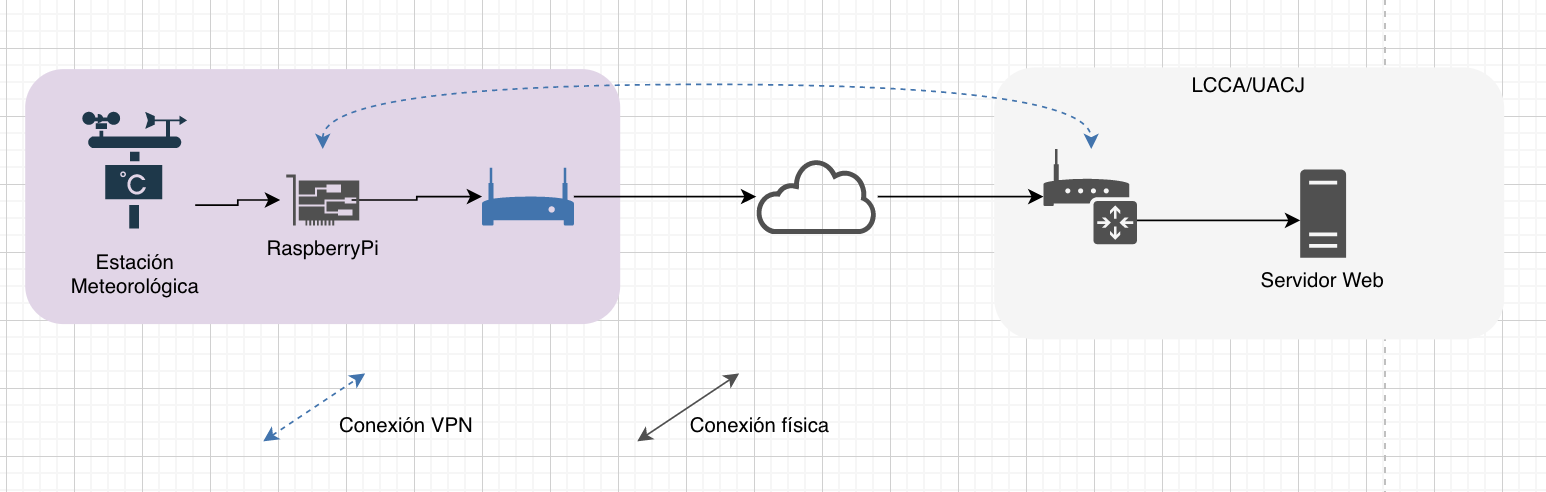
\includegraphics[width=.45\linewidth]{images/diagrams/conexion.png}
	\caption{Diagrama de la redundancia de las conexiones}
	\label{fig:conexion_redundancia}
\end{figure}

Por esta razón se optó por tener un servicio de monitoreo bidireccional. Se pretende que cambiando el ejecutor de servicios, se pueda obtener la información de la estación meteorológica sin necesidad de realizar diferentes implementaciones para cada caso. En este caso, se pretende que un script funcione en el mismo

\subsubsection{Consideraciones de seguridad}

Debido a que generalmente no se crea una red virtual privada separada para el manejo exclusivo de estaciones meteorológicas (ya que estas suelen instalarse sobre infraestructura existente) es importante tener consideraciones de seguridad respecto a el acceso a las estaciones, debido a que pueden ser un punto de acceso a una, otherwise, isolada y segura red.


\textbf{De la conexión del servidor a las estaciones meteorológicas}

Para realizar la conexión a las estaciones meteorológicas se requiere de acceso a la raspberrypi que funciona como puente entre ambas. Para realizar cambios, crear un servicio, y establecer la información del sistema con una mínima interacción se requiere de un usuario de alta prioridad a la máquina. En el caso del sistema operativo basado en linux que utilizan las estaciones, es el usuario con la mayor cantidad de procesos \emph{root}.

Al considerarse comprometido el ambiente de la apliación, se consideraría comprometido el sistema completo. Ya que en este ambiente se encontrarán las contraseñas de acceso a la base de datos y la llave privada que se utiliza para hacer autenticación, si bien existen servicios como Aws-KMS (Key Management Service), el implementar un sistema tan robusto para la administración de secretos sale de los objetivos de este proyecto.

Por lo tanto, se decidió crear un servicio que tome un usuario y password con acceso "root" de forma temporal (o al menos uno que tenga permisos de \emph{sudoer}) y utilizarlo para almacenar la llave pública local del servidor para realizar operaciones sin tener un usuario/password almacenado en la base de datos que pudiera ser comprometido. De esta forma, se mitiga el impacto de una posible intrusión a la base de datos, para no comprometer las credenciales de acceso a las estaciones.

\textbf{De las estaciones meteorológicas al servidor}

Debido a que las estaciones meteorológicas suelen ser instaladas en puntos con poco o mínimo control de seguridad física, se busca mitigar el acceso de las estaciones meteorológicas a la base de datos en la que se centralizarán los datos. Por lo tanto, se decidió utilizar un protocolo de API para insertar los eventos.

\subsection{Diseño de base de datos}





\subsubsection{Selección del motor de base de datos}

Para el caso de uso del centro de monitoreo de estaciones meteorológicas de la UACJ, en el que la red actual cuenta con 13 estaciones, no es necesario considerar como cuello de botella el motor de base de datos que se utilizará para el sistema. Esto debido a que, con un tiempo mínimo para la consulta del estado de las estaciones de hasta 5 minutos entre consultas, el sistema podría funcionar incluso con un motor de 23 segundos entre consultas.

Debido a que la infraestructura del sistema de las estaciones meteorológicas ya corre en un motor relacional adecuado para el proyecto, MySQL, se pretende utilizarlo para este proyecto, reduciendo la carga de mantenimiento al tener el sistema centralizado y proveyendo una facilidad para ser integrado con otros sistemas de ser necesario.

Para esto, se utilizó la flexibilidad que ofrecen los sistemas ORM (modelado de objetos y roles, por sus siglas en inglés) \cite{Halpin2006}, en la que se permite el crear sistemas agnósticos de un motor de base de datos en específico, y la creación de modelos, esquemas y relaciones de base de datos se dejan al sistema. Esto además ofrece soporte para migraciones para realizar actualizaciones de base de datos controladas en caso de requerir extender un sistema existente.



\subsection{Configuración de ambiente de
desarrollo}\label{configuraciuxf3n-de-ambiente-de-desarrollo}

El ambiente de desarrollo que se seleccionó para el proyecto fué
seleccionado con el objetivo de

\subsection{\texorpdfstring{Contenedor \emph{docker} para
desarrollo}{Contenedor docker para desarrollo}}\label{contenedor-docker-para-desarrollo}

Con la finalidad de tener un contenedor de desarrollo que pueda ser
replicado con la mínima configuración se eligió la plataforma docker,
por su amplia adopción y por las facilidades que ofrece para crear
sistemas complejos que dependen de varios servicios sin tener que
realizar configuraciones en el sistema que puedan ser perdidas al
momento de cambiar a otro.

Debido a la sencillez que el sistema de cnfiguración de contenedores
\emph{docker compose} ofrece, se eligió para almacenar los parámetros de
configuración de los contenedores en vez de crear comandos compatibles
con docker para ello. Esto permite una fácil edición de los servicios y
la aplicación de los mismos de una forma estandarizada que permite la
fácil lectura de los parámetros.

El archivo de configuración fué almacenado en la raíz del proyecto, con
el nombre de \texttt{docker-compose.yml} tal como el estándar de la
utilería \texttt{docker-compose} sugiere, y este archivo tiene el
contenido siguiente que se muestra en el listado {[}INSERTAR{]}.

\begin{Shaded}
\begin{Highlighting}[]
\FunctionTok{version}\KeywordTok{:}\AttributeTok{ }\StringTok{\textquotesingle{}3.3\textquotesingle{}}

\FunctionTok{services}\KeywordTok{:}
\AttributeTok{  }\FunctionTok{mysql}\KeywordTok{:}
\AttributeTok{    }\FunctionTok{image}\KeywordTok{:}\AttributeTok{ mysql}
\AttributeTok{    }\FunctionTok{container\_name}\KeywordTok{:}\AttributeTok{ meteoreo{-}mysql}
\AttributeTok{    }\FunctionTok{environment}\KeywordTok{:}
\AttributeTok{      }\FunctionTok{MYSQL\_DATABASE}\KeywordTok{:}\AttributeTok{ $\{MYSQL\_DATABASE\}}
\AttributeTok{      }\FunctionTok{MYSQL\_ROOT\_PASSWORD}\KeywordTok{:}\AttributeTok{ $\{MYSQL\_ROOT\_PASSWORD\}}
\AttributeTok{      }\FunctionTok{MYSQL\_PASSWORD}\KeywordTok{:}\AttributeTok{ $\{MYSQL\_PASSWORD\}}
\AttributeTok{      }\FunctionTok{MYSQL\_USER}\KeywordTok{:}\AttributeTok{ $\{MYSQL\_USER\}}
\AttributeTok{      }\FunctionTok{SERVICE\_TAGS}\KeywordTok{:}\AttributeTok{ dev}
\AttributeTok{      }\FunctionTok{SERVICE\_NAME}\KeywordTok{:}\AttributeTok{ mysql}
\AttributeTok{    }\FunctionTok{ports}\KeywordTok{:}
\AttributeTok{      }\KeywordTok{{-}}\AttributeTok{ }\StringTok{"3306:3306"}
\AttributeTok{    }\FunctionTok{networks}\KeywordTok{:}
\AttributeTok{      }\KeywordTok{{-}}\AttributeTok{ meteoreo{-}backend}

\AttributeTok{  }\FunctionTok{api}\KeywordTok{:}
\AttributeTok{    }\FunctionTok{container\_name}\KeywordTok{:}\AttributeTok{ meteoreo{-}api}
\AttributeTok{    }\FunctionTok{build}\KeywordTok{:}
\AttributeTok{      }\FunctionTok{context}\KeywordTok{:}\AttributeTok{ ./}
\AttributeTok{      }\FunctionTok{dockerfile}\KeywordTok{:}\AttributeTok{ Dockerfile}
\AttributeTok{    }\FunctionTok{volumes}\KeywordTok{:}
\AttributeTok{      }\KeywordTok{{-}}\AttributeTok{ }\StringTok{\textquotesingle{}./:/app:delegated\textquotesingle{}}
\AttributeTok{    }\FunctionTok{depends\_on}\KeywordTok{:}
\AttributeTok{      }\KeywordTok{{-}}\AttributeTok{ mysql}
\AttributeTok{    }\FunctionTok{environment}\KeywordTok{:}
\AttributeTok{      }\KeywordTok{{-}}\AttributeTok{ WEB\_CONCURRENCY=2}
\AttributeTok{      }\KeywordTok{{-}}\AttributeTok{ PORT=80}
\AttributeTok{      }\KeywordTok{{-}}\AttributeTok{ PRE\_START\_PATH=/app/app/prestart.sh}
\AttributeTok{      }\KeywordTok{{-}}\AttributeTok{ GUNICORN\_CMD\_ARGS="{-}{-}reload"}
\AttributeTok{    }\FunctionTok{ports}\KeywordTok{:}
\AttributeTok{      }\KeywordTok{{-}}\AttributeTok{ }\StringTok{"81:80"}
\AttributeTok{    }\FunctionTok{networks}\KeywordTok{:}
\AttributeTok{      }\KeywordTok{{-}}\AttributeTok{ meteoreo{-}backend}

\FunctionTok{networks}\KeywordTok{:}
\AttributeTok{  }\FunctionTok{meteoreo{-}backend}\KeywordTok{:}
\AttributeTok{    }\FunctionTok{driver}\KeywordTok{:}\AttributeTok{ bridge}
\end{Highlighting}
\end{Shaded}

Las variables utilizadas para el sistema vienen del archivo
\texttt{.env} en la raíz del proyecto. Estas variables tienen el

\subsection{\texorpdfstring{\emph{Devcontainer}}{Devcontainer}}\label{devcontainer}

Para tener una plataforma de desarrollo sencilla de configurar para
proveer la máxima compatibilidad de se utilizó de una herramienta
relativamente común en el desarrollo de aplicaciones con Visual Studio
Code, el uso de \emph{devcontainers}. Estos son, un archivo de
configuración que da indicaciones al editor de código para crear un
ambiente a la medida dentro de un contenedor docker.

Para realizar la configuración de este contenedor, se creó un directorio
en la raíz del repositorio* llamado \texttt{.devcontainer}, y dentro de
este folder se puso un archivo \texttt{devcontainer.json} como se
muestra en el listado {[}LISTADO{]}

\begin{Shaded}
\begin{Highlighting}[]
\FunctionTok{\{}
  \DataTypeTok{"name"}\FunctionTok{:} \StringTok{"Meteoreo API"}\FunctionTok{,}
  \DataTypeTok{"service"}\FunctionTok{:} \StringTok{"api"}\FunctionTok{,}
  \DataTypeTok{"remoteUser"}\FunctionTok{:} \StringTok{"root"}\FunctionTok{,}
  \DataTypeTok{"shutdownAction"}\FunctionTok{:} \StringTok{"stopCompose"}\FunctionTok{,}
  \DataTypeTok{"workspaceFolder"}\FunctionTok{:} \StringTok{"/app"}\FunctionTok{,}
  \DataTypeTok{"dockerComposeFile"}\FunctionTok{:} \StringTok{"../docker{-}compose.yml"}\FunctionTok{,}
  \DataTypeTok{"extensions"}\FunctionTok{:} \OtherTok{[}
	 \StringTok{"editorconfig.editorconfig"}\OtherTok{,}
	 \StringTok{"mikestead.dotenv"}\OtherTok{,}
	 \StringTok{"njpwerner.autodocstring"}\OtherTok{,}
	 \StringTok{"aaron{-}bond.better{-}comments"}\OtherTok{,}
	 \StringTok{"mhutchie.git{-}graph"}\OtherTok{,}
	 \StringTok{"hookyqr.beautify"}\OtherTok{,}
	 \StringTok{"magicstack.magicpython"}\OtherTok{,}
	 \StringTok{"gruntfuggly.todo{-}tree"}\OtherTok{,}
	 \StringTok{"ms{-}python.vscode{-}pylance"}\OtherTok{,}
	 \StringTok{"sleistner.vscode{-}fileutils"}
	\OtherTok{]}
\FunctionTok{\}}
\end{Highlighting}
\end{Shaded}

En este archivo se especifica un nombre para identificar el ambiente de
desarrollo que sea reconocible por el desarrollador, la localización del
archivo que describe el contenedor, y una lista de extensiones para el
editor de código. Entre las más importantes se encuentra \emph{pylance}
y \emph{magicpython}, las demás son meramente preferencias personales
para el ambiente de programación.


\section{Módulo de monitoreo de estaciones meteorológicas}





\section{Selección de base de datos}

%! Terminar para la próxima

% Casi todas las secciones de desrrollo, van ligadas a una de resultados.

%? Escribir el proceso que realicé. Presentar lo suficiente para darle una idea al lector.

%? Presentar un fragmento de código más relevante. Incluir enlace a repositorio. La funcionalidad se puede expresar en algún tipo de representación gráfica.

%? Evitar párrafos de una sola oración. (Dar MÁS contexto), extranjerismos en itálica.
Con un tiempo de respuesta de $~[N]ms$, el sistema puede soprotar hasta N estaciones concurrentes.

Debido a que la recolección de los datos es por métodología pull y no push, es posible tener las estaciones en una cola que se ejecute hasta por un periodo de 5 minutos (que es un estándar en la recolección de datos de estaciones meteorológicas). Esto implica que la base de datos [X] puede soportar hasta [N x 60 x 5] datos de forma concurrente.

Tomando en cuenta las necesidades actuales del LCCA, y el estimado del tamaño de las redes de alta densidad (que pueden llegar hasta los N nodos como X artículo lo demuestra), no vale la pena el introducir la complejidad extra de un motor de base de datos desconocido y para el que no existen ORM's con soporte completo en el lenguaje de desarrollo. Porque no es un sistema de alta densidad de datos.

Si bien es posible escalar horizontalmente la infraestructura, se busca evitarlo ya que los \textit{diminishing returns} del costo de tener que mantener un sistema de monitoreo no es costeable. Para los casos de sistemas de extremadamente alta densidad, se recomienda el crear varias instancias seccionadas en bases de datos, o escalar la base de con un redis en vez de escalar.

%! Recordar que la información debe ser consultada desde el API, así que no sólo se tienen que tomar en cuenta la cantidad de query's por segundo que se requieren hacer para las inserciones, sino también para la consulta de datos.

%! Si lo que queremos es proveer herramientas para la gestión de calidad de los datos meteorológicos, la información tiene que tener en mente los principios Solidos y transaccionales, al menos en la creación de reportes basados en incidentes.


\section{Avances}


\section{Módulo de monitoreo}

\subsection*{Requisitos}

\subsection*{Seguridad}

\subsection*{Método de conexion}
